\documentclass{article}


% if you need to pass options to natbib, use, e.g.:
%     \PassOptionsToPackage{numbers, compress}{natbib}
% before loading neurips_2024


% ready for submission
% \usepackage[final]{neurips_2024}


% to compile a preprint version, e.g., for submission to arXiv, add add the
% [preprint] option:
    \usepackage[preprint]{neurips_2024}


% to compile a camera-ready version, add the [final] option, e.g.:
%    \usepackage[final]{neurips_2024}


% to avoid loading the natbib package, add option nonatbib:
%    \usepackage[nonatbib]{neurips_2024}


\usepackage[utf8]{inputenc} % allow utf-8 input
\usepackage[T1]{fontenc}    % use 8-bit T1 fonts
\usepackage{hyperref}       % hyperlinks
\usepackage{url}            % simple URL typesetting
\usepackage{booktabs}       % professional-quality tables
\usepackage{amsfonts}       % blackboard math symbols
\usepackage{nicefrac}       % compact symbols for 1/2, etc.
\usepackage{microtype}      % microtypography
\usepackage{xcolor}         % colors
\usepackage{amsmath}
\usepackage{graphicx}
\usepackage{float}


\title{Assignment-12 : Neural Networks}


% The \author macro works with any number of authors. There are two commands
% used to separate the names and addresses of multiple authors: \And and \AND.
%
% Using \And between authors leaves it to LaTeX to determine where to break the
% lines. Using \AND forces a line break at that point. So, if LaTeX puts 3 of 4
% authors names on the first line, and the last on the second line, try using
% \AND instead of \And before the third author name.


\author{Harshvardhan Patidar\\
  Department of Artificial Intelligence\\
  Indian Institute of Technology Hyderabad\\
  \texttt{ai24btech11015@iith.ac.in}
  % example of co authors
  % \And
  % Coauthor \\
  % Affiliation \\
  % Address \\
}


\begin{document}\



\maketitle



%If you want to add an abstract, use below commands
%\begin{abstract}
%\end{abstract}



%use below command to get heading
%\section{Heading}

%If you don't want it to be included in the index, use
%\section*{}



%use below command to get sub-heading sort of thing
%\subsection{Style}



%use below commands for centering and url accordingly
%\begin{center}
%  \url{http://www.neurips.cc/}
%\end{center}



%Use below commmand for creating new paragraph
%\paragraph{}



%You can use below commands in the text to refer to specific sections (you need to use /label{} to where you are referring 
%\ref{gen_inst}



%use below to have nice tiny inline fractions, to increase space between them, use a tildae as in the latter
%\nicefrac{1}{4} Hello this is harshvardhan, typing his latex assignments
%\nicefrac{1}{4}~ Hello this is harshvardhan, typing his latex assignments



%for adding a footnote (vo jo page ke niche hi niche aate hai)
%\footnote{As in this example.}



%For adding a photo/figure
%\begin{figure}
%  \centering
%  \fbox{\rule[-.5cm]{0cm}{4cm} \rule[-.5cm]{4cm}{0cm}}
%  \caption{Sample figure caption.}
%\end{figure}



%For a table	
%\begin{table}
%  \caption{Sample table title}
%  \label{sample-table}
%  \centering
%  \begin{tabular}{lll}
%    \toprule
%    \multicolumn{2}{c}{Part}                   \\
%    \cmidrule(r){1-2}
%    Name     & Description     & Size ($\mu$m) \\
%    \midrule
%    Dendrite & Input terminal  & $\sim$100     \\
%    Axon     & Output terminal & $\sim$10      \\
%    Soma     & Cell body       & up to $10^6$  \\
%    \bottomrule
%  \end{tabular}
%\end{table}



%use for a giving a vertical space 
%\medskip



%Use for appendix (idk what it is)
%\appendix



%For yes, no or na
%You should answer \answerYes{}, \answerNo{}, or \answerNA{}.

\section{Deep Learning}
  \paragraph{} Deep learning is a family of techniques of machine learning in which the hypotheses are represented by complex algebraic circuits, with configurable connection strength of each connection. The word “deep” is to refer to the fact that the circuits are organized into many layers, or simply the computation path of input to output consists of a lot of steps. One of the very first implementations of deep learning was to make an artificial model network of neurons like in the brain, in the form of computational circuits by McCulloch and Pitts in 1943. This is in fact the reason why the networks trained by the technique of deep learning are called neural networks. 
  \paragraph{} Now the question arises, why Deep learning has advantages over the earlier discussed linear techniques. The reason is that even though the linear and logistic regression can take in a large number of inputs, the computation path is very short, and each input contributes individually to the output. This causes their expressive power to become limited. Which causes it to fail to represent the real-word complex scenarios.
  \paragraph{} Decision lists and decision trees also don’t fulfill the criteria as even though they allow long computation paths, the number of input vectors is relatively small. Deep learning takes advantage here by making all the input variables interact with each other in a complex manner. The models developed by this method are sufficiently expressive to represent the real-word complex data.
  
  \subsection{Simple Feedforward Networks}
    \paragraph{} The feedforward networks have connections only in one direction. Each node takes the input, computes the corresponding output and then passes that output to the next node in the network. No closed loops are formed in such networks. Whereas, in a recurrent network, the intermediate or final outputs are feeded back into its inputs. This arranges the signal values in a dynamical system maintaining its own internal state and memory.
    \paragraph{} Boolean circuits are a good example of feedforward networks, in which the inputs and the outputs are limited to 0 and 1. In neural networks, typically the input values are continuous and produce continuous outputs. In such models, some of the inputs play the roles of parameters. The model learns by configuring these parameters, so that the network best fits the training data.
    \subsubsection{Networks as complex functions}
      \paragraph{} Each node in the network is termed as an unit. It follows the traditional design given by McCulloch and Pitts, in which a unit calculates the weighted sum of the inputs from its previous nodes, then applies some non-linear function to produce the output. Let $a_j$ denote the output of unit $j$ and let $w_{i,j}$ be the weight corresponding to the link	from unit $i$ to unit $j$, then
      \begin{equation*}
        a_j = g_j (\textit{i} n_j) \equiv g_j ( \sum_i w_{i,j} a_j)
      \end{equation*}
      where $g_j$ is the nonlinear activation function, for unit $j$ an $\textit{i} n_j$ denotes the weighted sum of the inputs to the unit. As we did earlier, we will add an extra dummy unit 0 with a fixed value of 1 and a weight $w_{0,j}$ for that input. This makes our total weighted input remain non-zero. The previous equation can be rewritten as
      \begin{equation*}
        a_j = g_j (\mathbf{w}^{\top} \mathbf{x})
      \end{equation*}
      It is important to note that the activation function $g_j$ is nonlinear because if it were not, then any composition of the units and functions would only represent the linear functions and hence have limited expressive power. The universal approximation, states that a network with as low as two layers of computational units can approximate any continuous function to an arbitrary degree of accuracy.

      \paragraph{} A great variety of activation functions are used depending on the type of problem. Some of them are :
      \begin{itemize}
        \item The logistic or the \textbf{sigmoid} function which we discussed in the previous assignment on logistic regression
	        \begin{equation*}
		        \sigma (x) = 1 / (1 + e^{-x})
	        \end{equation*}

          \item The \textbf{ReLU} function. (abbreviated form of rectified linear unit):
          \begin{equation*}
            \text{ReLU}(x) = \text{max}(0,x)
          \end{equation*}

          \item The \textbf{softplus} function, a smoother version of the ReLU function:
	          \begin{equation*}
		          \text{softplus}(x) = \log{1+ e^x}
	          \end{equation*}
            It is important to note that the sigmoid function is the derivative of the softplus function.

            \item The \textbf{tanh} function
            \begin{equation*}
              \tanh (x) = \frac{e^{2x} -1}{e^{2x} + 1}
            \end{equation*}
              
            \begin{figure}[H]
              \centering
              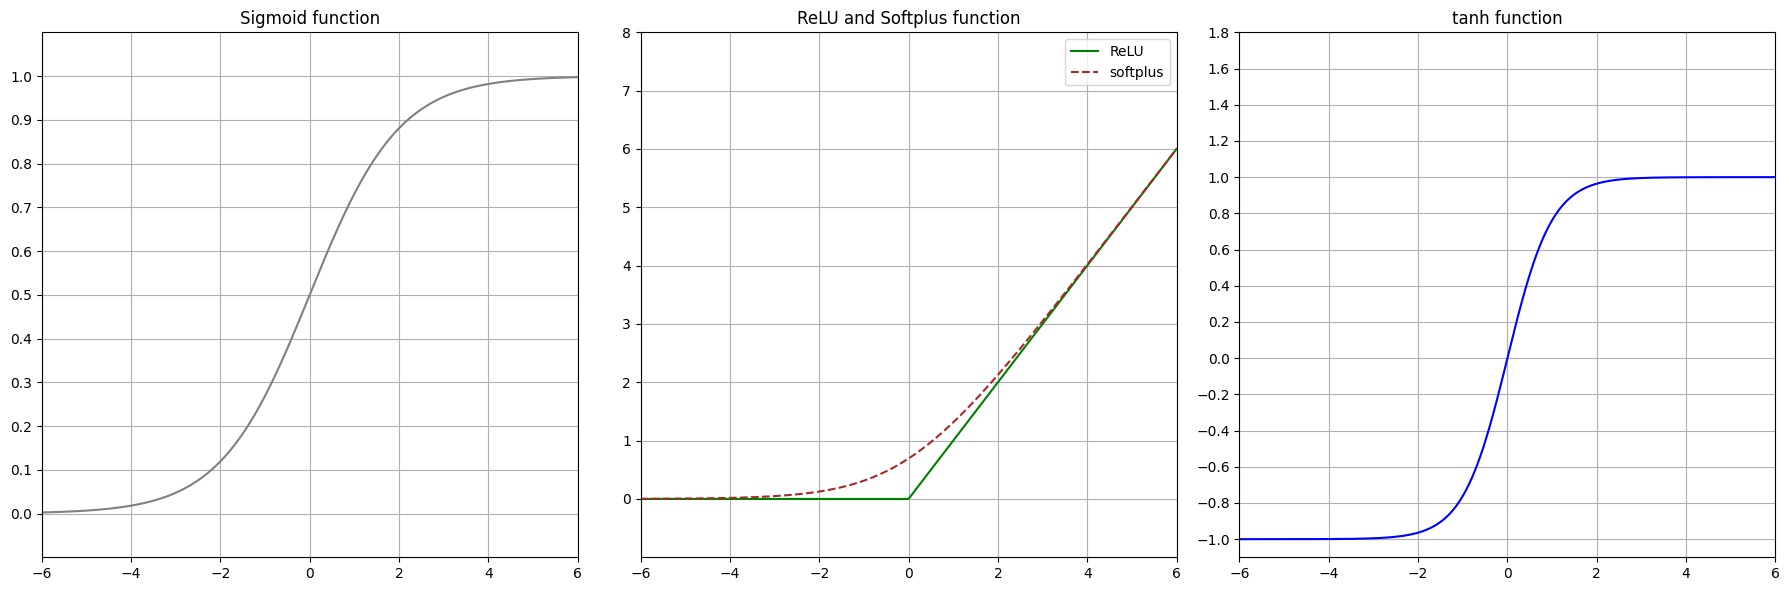
\includegraphics[width=1\textwidth]{plot.png}
              \caption{Common Activation Functions}
           \end{figure}

           
      \end{itemize}

      \paragraph{} An expression for the output $\hat{y}$ can be written as 
           \begin{align*}
            \hat{y} &= g_5(\text{in}_5) = g_5(w_{0,5} + w_{3,5}a_3 + w_{4,5}a_4)\\
            &= g_5(w_{0,5} + w_{3,5}g_3(\text{in}_3) + w_{4,5}g_4(\text{in}_4))\\
            &= g_5(w_{0,5} + w_{3,5}g_3(w_{0,3} + w_{1,3}x_1 + w_{2,3}x_2)
            + w_{4,5}g_4(w_{0,4} + w_{1,4}x_1 + w_{2,4}x_2))
           \end{align*}

           \newpage

           \begin{figure}[H]
            \centering
            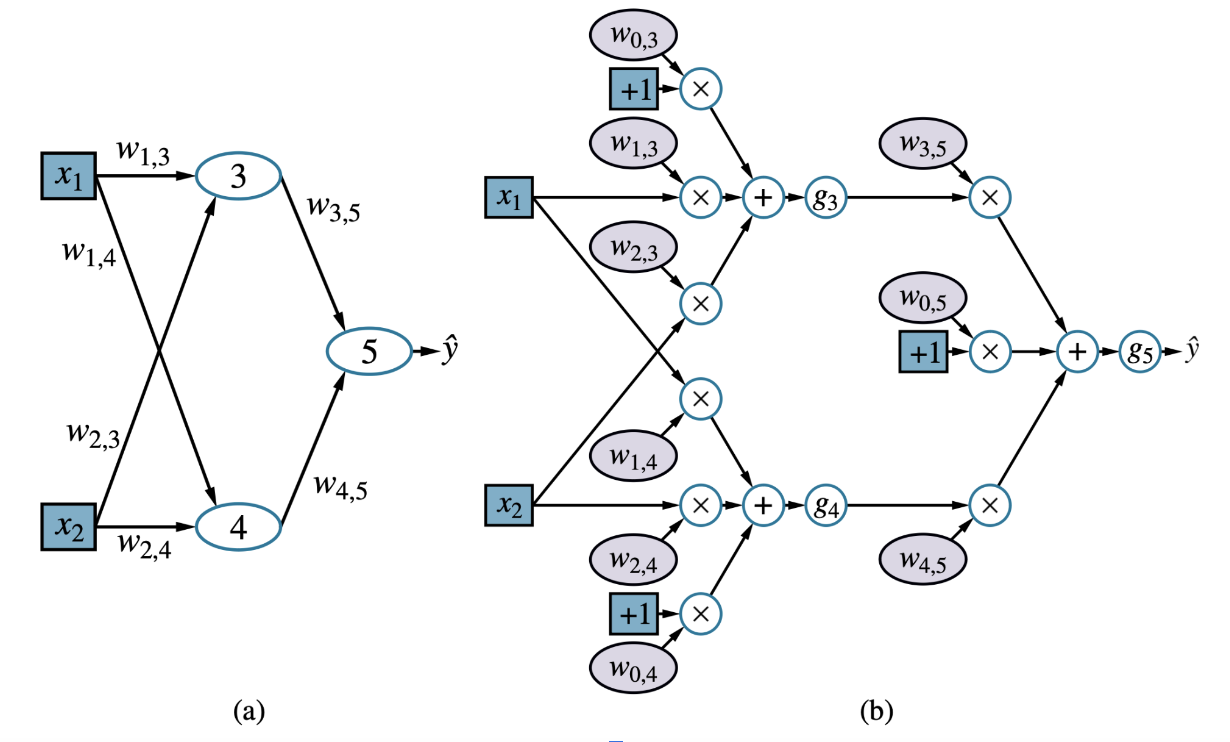
\includegraphics[width=1\textwidth]{ss.png}
            \caption{Graph of neural network}
         \end{figure}

         The general way (b) to represent the network is called the computation graph or the dataflow graph. These are circuits in which each node represents an elementary computation.
         To represent the network in matrix form to make it easy to work on in computers, we denote \textbf{W} to denote the weight matrix. For the network in figure, $\textbf{W}^{(1)}$ denotes the weight of the first layer $(w_{1,3}, w_{1,4},\ldots)$ and $\textbf{W}^{(2)}$ denotes the weights in the second layer. Let $\textbf{g}^{(1)}$ and $\textbf{g}^{(2)}$ denote the activation function in the first and second layers, then the network can be written as
         \begin{equation*}
          \mathbf{h}(x) = \mathbf{g}^{(2)}\left(\mathbf{W}^{(2)}\mathbf{g}^{(1)}\left(\mathbf{W}^{(1)}\mathbf{x}\right)\right).
         \end{equation*}

         This expression corresponds to a computation graph, much simpler than in  Figure 2(b). The graph in Figure 2(b) is relatively very small and shallow, but the same concept is applied in large and more complex models. The figure is also fully connected, which means that every node in each layer is connected to every node in the next layer.
    \subsubsection{Gradients and Learning}
    \paragraph{} In the linear regression, we used the gradient descent algorithm to find the best hypothesis. We can apply the same algorithm here to find the best model. For the weights leading into the output layer, the process is identical to what we did earlier, but for the weights leading to the hidden layer, we need to use the chain rule to get to the gradient. We will consider the squared loss function $(L_2)$
    \begin{equation*}
      \textit{Loss}(h_\mathbf{w}) = L_2(y, h_{\mathbf{w}}(\mathbf{x})) = \| y - h_{\mathbf{w}}(\mathbf{x}) \|^2 = (y - \hat{y})^2
    \end{equation*}

    \paragraph{} The gradient calculations are below
    \begin{align*}
      \frac{\partial}{\partial w_{3,5}} \emph{Loss}(h_{\mathbf{w}}) &= \frac{\partial}{\partial w_{3,5}} (y - \hat{y})^2 \\
      &= -2 (y - \hat{y}) \frac{\partial \hat{y}}{\partial w_{3,5}} \\
      &= -2 (y - \hat{y}) \frac{\partial}{\partial w_{3,5}} g_5(in_5) \\
      &= -2 (y - \hat{y}) g_5'(in_5) \frac{\partial in_5}{\partial w_{3,5}} \\
      &= -2 (y - \hat{y}) g_5'(in_5) \frac{\partial}{\partial w_{3,5}} (w_{0,5} + w_{3,5}a_3 + w_{4,5}a_4) \\
      &= -2 (y - \hat{y}) g_5'(in_5) a_3.
    \end{align*}

    This calculation was easy as $w_{0,5}$ and $w_{4,5}a_4$ do not depend on $w_{3,5}$. The more complex case might involve weights such as $w_{1,3}$, which are not directly to the output layer, so we need to apply chain rule for this one more time.

    \begin{align*}
      \frac{\partial}{\partial w_{1,3}} \emph{Loss}(h_{\mathbf{w}}) &= -2 (y - \hat{y}) g_5'(in_5) \frac{\partial}{\partial w_{1,3}} (w_{0,5} + w_{3,5}a_3 + w_{4,5}a_4) \\
      &= -2 (y - \hat{y}) g_5'(in_5) w_{3,5} \frac{\partial a_3}{\partial w_{1,3}} \\
      &= -2 (y - \hat{y}) g_5'(in_5) w_{3,5} g_3'(in_3) \frac{\partial in_3}{\partial w_{1,3}} \\
      &= -2 (y - \hat{y}) g_5'(in_5) w_{3,5} g_3'(in_3) \frac{\partial}{\partial w_{1,3}} (w_{0,3} + w_{1,3}x_1 + w_{2,3}x_2) \\
      &= -2 (y - \hat{y}) g_5'(in_5) w_{3,5} g_3'(in_3) x_1.
    \end{align*}

    Now, we will try to understand the term back-propagation.

    \begin{itemize}
      \item \textbf{For unit 5}: The error is given as $\Delta_5 = 2(\hat{y} - y)g'_5(in_5)$ and the gradient w.r.t  $w_{3,5}$ is $\frac{\partial}{\partial w_{3,5}} = \Delta_5 a_3$. This means the error is scaled by the input $a_3$. If both $\Delta_5$ and $a_3$ have the same sign, increasing $w_{3,5}$ increases the error, while if it has opposite signs then it is decreased.
      \item \textbf{For unit 3}: The error at unit 5 is propagating backward, contributing to error at unit 3. This is given by $\Delta_3 = \Delta_5 w_{3,5} g'_3(in_3)$. The gradient with respect to $w_{1,3}$ is $\frac{\partial}{\partial w_{1,3}} = \Delta_3 x_1$, evident of the fact that the error at unit 5 is scaled by $w_{3,5}$, the activation gradient at unit 3, and the input $x_1$. 
    \end{itemize}

    This phenomenon gives rise to the term back-propagation as the error at output is being passed back through the network
    \paragraph{} The derivations we did above are just for illustration purposes and we don’t need to do them ourselves while training a model. All such gradients can be calculated by the technique of automatic differentiation. All the major packages provide automatic differentiation. So the user does not need to do such complex computations, and can be more focused on training the model better.  

\newpage
\section{Computation Graphs for Deep Learning}
  \paragraph{} We will look at how to put together computation graphs and tune the weights by computing the gradient to make our model best-fit the data.
    \subsection{Input Encoding}
      \paragraph{} The input and output nodes are those which are connected directly to the input and output. For factored data, the encoding is pretty straightforward as each training example contains values of the $n$ input attributes. But  image data doesn’t fit well in the category of factored data. If we have a fully connected model for these, then the importance of adjacency of pixels will be lost. For this reason, in the hidden layers, they aren’t completely interconnected, but connected to only a few adjacent pixels. For categorical attributes, where multiple possible attributes are possible, we represent it by $d$ separate input bits, with the bit of chosen one being 1 and the others being 0. We can't use $1,2,3 \ldots$ to represent the options as the difference between 1\& 2 and that between 1\& 3 are different but this doesn't make sense.
    \subsection{Output Encoding}
      \paragraph{} After output encoding, now we need to represent the output into  actual meaningful categories. One example could be again using reverse of one-hot encoding. More importantly, for the loss, we will treat the output values as probabilities instead of values (like in the negative log likelihood loss function). In Deep learning we commonly use the term cross-entropy and try to minimize this. It is denoted as \textit{H(P, Q)} is a measure of dissimilarity between \textit{P} and \textit{Q}. Here \textit{P} is the true distribution over the training examples, whereas \textit{Q} is for the predictive hypotheses.
      \paragraph{} Sometimes, to denote the data in the form of probabilities, we use the softmax layer, which gives the probability according to the given inputs. It outputs a vector of $d$ values for a given input vector $\mathbf{in} = \langle in_1, \dots, in_d \rangle$, where the $k^{th}$ element is
      \begin{equation*}
        \text{softmax}(\mathbf{in})_k = \frac{e^{in_k}}{\sum_{k' = 1}^{d} e^{in_{k'}}}
      \end{equation*}

      The softmax outputs a vector of non-negative values which sum up to 1. These probabilities are then used to minimize the cross entropy and hence to train the model.



\end{document}
